\documentclass[tikz,border=8pt]{standalone}
\usepackage{tikz}
\usepackage{xcolor}
\usepackage{amsmath}
\usetikzlibrary{shapes.geometric, positioning, calc}

%% ── Colours ──────────────────────────────────────────────────────────────────
\definecolor{rootbg}   {HTML}{E9EFF5}
\definecolor{rootbdr}  {HTML}{91A4B7}
\definecolor{trunkclr} {HTML}{9AA8B5}
\definecolor{leafbdr}  {HTML}{d3d1c7}
\definecolor{leaftxt}  {HTML}{3d3d3a}

% Axis header colours (bg / border / text)
\definecolor{ax1bg}  {HTML}{EEF2FF} \definecolor{ax1bd}  {HTML}{7788CF} \definecolor{ax1tx}  {HTML}{2E3C7B}
\definecolor{ax2bg}  {HTML}{E6F4F0} \definecolor{ax2bd}  {HTML}{5A9D89} \definecolor{ax2tx}  {HTML}{225C4E}
\definecolor{ax3bg}  {HTML}{FCF1E2} \definecolor{ax3bd}  {HTML}{BE8C4A} \definecolor{ax3tx}  {HTML}{6C4517}
\definecolor{ax4bg}  {HTML}{FCEEEA} \definecolor{ax4bd}  {HTML}{C17B64} \definecolor{ax4tx}  {HTML}{7A3F2F}
\definecolor{ax5bg}  {HTML}{EAF2FB} \definecolor{ax5bd}  {HTML}{7297BC} \definecolor{ax5tx}  {HTML}{27496B}
\definecolor{ax6bg}  {HTML}{EDF5E5} \definecolor{ax6bd}  {HTML}{85A163} \definecolor{ax6tx}  {HTML}{415B24}

% Method colours
\definecolor{cwanda}    {HTML}{2F6DA3}
\definecolor{csparsegpt}{HTML}{2F7D68}
\definecolor{cmrp}      {HTML}{A36A2D}
\definecolor{cllmp}     {HTML}{A14D67}
\definecolor{cziplm}    {HTML}{5E7E2F}
\definecolor{cevopress} {HTML}{5F6FCB}

%% ── Symbol macros (inline TikZ pictures) ────────────────────────────────────
\newcommand{\symWanda}{\tikz[baseline=-1pt]\fill[cwanda] (0,0) circle (3.5pt);}
\newcommand{\symSparseGPT}{\tikz[baseline=-1pt]\fill[csparsegpt] (-3pt,-3pt) rectangle (3pt,3pt);}
\newcommand{\symMRP}{\tikz[baseline=-1pt]\fill[cmrp] (0,4pt) -- (4pt,-3pt) -- (-4pt,-3pt) -- cycle;}
\newcommand{\symLLMP}{\tikz[baseline=-1pt]\fill[cllmp] (0,4pt) -- (4pt,0) -- (0,-4pt) -- (-4pt,0) -- cycle;}
\newcommand{\symZipLM}{\tikz[baseline=-1pt]
  \fill[cziplm] (0,5pt) -- (1.8pt,1.5pt) -- (5.5pt,1.5pt) -- (2.8pt,-0.8pt)
              -- (3.8pt,-4.5pt) -- (0,-2pt) -- (-3.8pt,-4.5pt)
              -- (-2.8pt,-0.8pt) -- (-5.5pt,1.5pt) -- (-1.8pt,1.5pt) -- cycle;}
\newcommand{\symEvoPr}{\tikz[baseline=-1pt]
  \fill[cevopress] (0,5pt) -- (4.5pt,2.5pt) -- (4.5pt,-2.5pt)
                 -- (0,-5pt) -- (-4.5pt,-2.5pt) -- (-4.5pt,2.5pt) -- cycle;}

%% ── Helpers ──────────────────────────────────────────────────────────────────
% Leaf node: \leafnode{text}{symbols}
% drawn at current scope's (0,0)
\newcommand{\leafnode}[2]{%
  \node[draw=leafbdr, fill=white, rounded corners=3pt,
        minimum width=3.1cm, minimum height=0.85cm,
        font=\small\color{leaftxt}, align=center,
        line width=0.4pt] (lf) {#1 \\ \footnotesize #2};
}

% Axis header: \axisheader{label}{bg}{bd}{tx}
\newcommand{\axisheader}[4]{%
  \node[draw=#3, fill=#2, rounded corners=4pt,
        minimum width=3.1cm, minimum height=0.75cm,
        font=\small\bfseries\color{#4}, align=center,
        line width=0.6pt] {#1};
}

\begin{document}
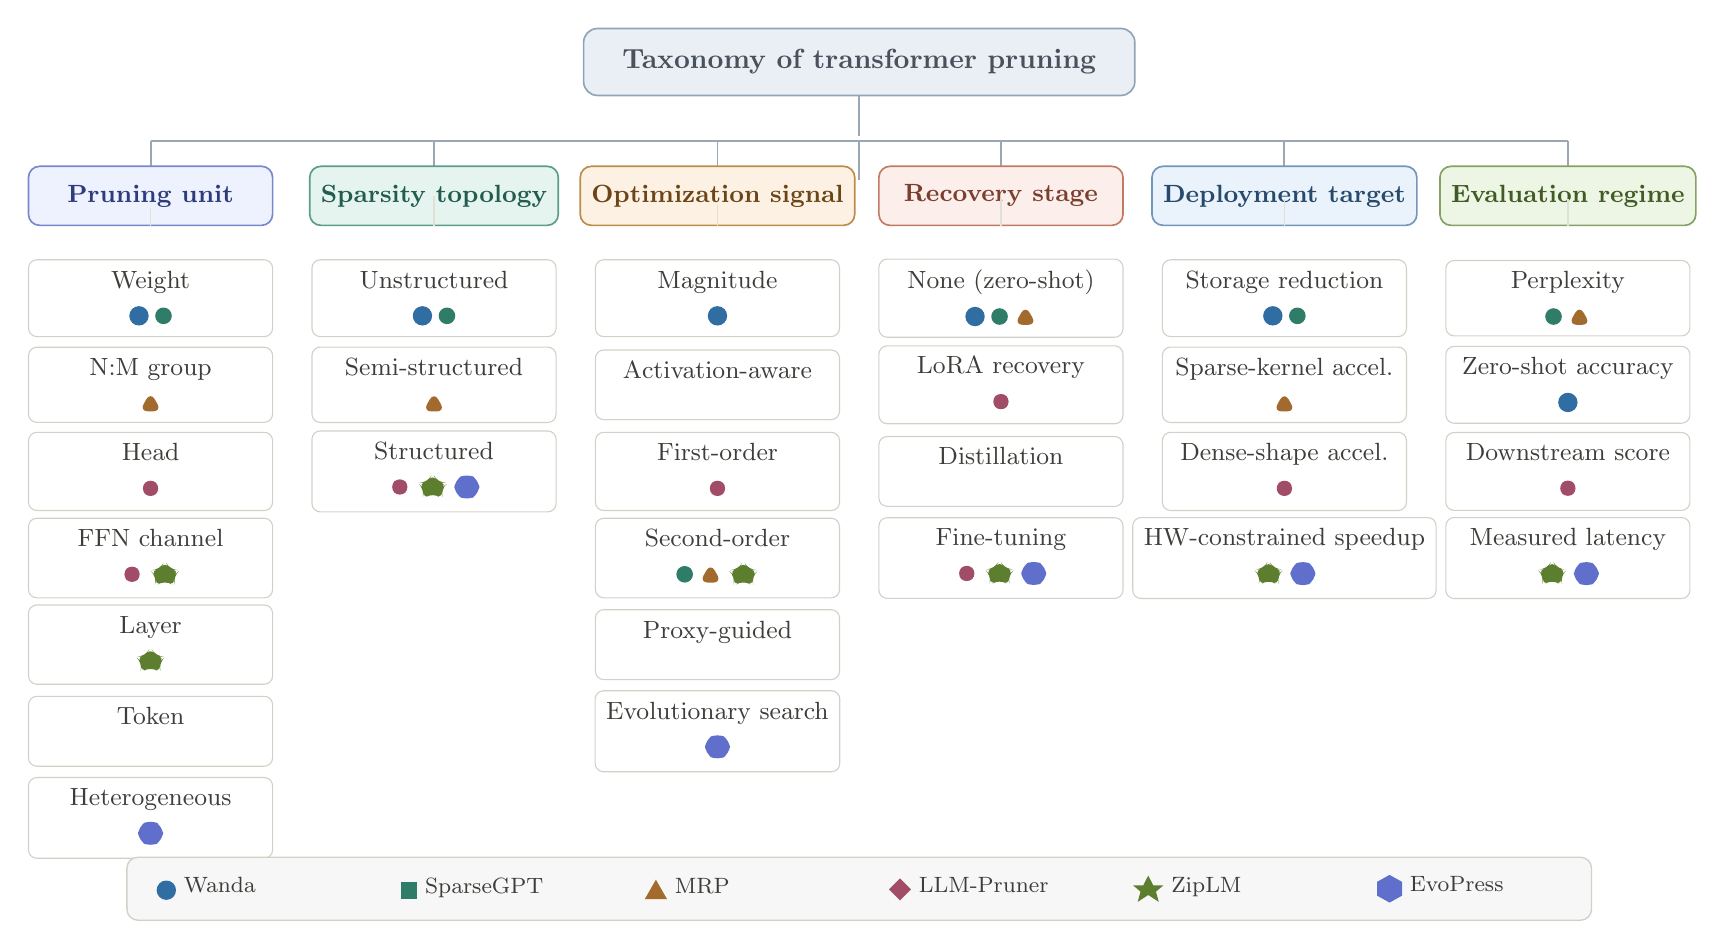
\begin{tikzpicture}[
  every node/.style={inner sep=4pt},
  font=\sffamily,
  ysep/.store in=\ysep, ysep=1.1cm,   % vertical gap between leaves
]

%% ── Layout constants ─────────────────────────────────────────────────────────
\def\rootY{0}
\def\trunkY{-1.0}   % y of horizontal trunk line
\def\headerY{-1.7}  % y of axis header centres
\def\firstY{-3.0}   % y of first leaf row
\def\rowstep{-1.1}  % step per leaf row

% Column x positions (6 columns)
\def\xI{0}
\def\xII{3.6}
\def\xIII{7.2}
\def\xIV{10.8}
\def\xV{14.4}
\def\xVI{18.0}

%% ══════════════════════════════════════════════════════════════════════════════
%%  ROOT
%% ══════════════════════════════════════════════════════════════════════════════
\node[draw=rootbdr, fill=rootbg, rounded corners=5pt,
      minimum width=7cm, minimum height=0.85cm,
      font=\normalsize\bfseries\color{rootbdr!50!black},
      line width=0.6pt] at (9.0,\rootY) (ROOT) {Taxonomy of transformer pruning};

%% Trunk: vertical drop then horizontal bar
\draw[trunkclr, line width=0.7pt]
  (ROOT.south) -- ++(0,-0.5) coordinate (trunkTop);
\draw[trunkclr, line width=0.7pt]
  (\xI,\trunkY) -- (\xVI,\trunkY);
% Drops to each column header
\foreach \cx in {\xI,\xII,\xIII,\xIV,\xV,\xVI} {
  \draw[trunkclr, line width=0.7pt] (\cx,\trunkY) -- (\cx,\headerY+0.375);
}
% Connect trunk top to horizontal bar
\draw[trunkclr, line width=0.7pt] (9.0,\trunkY-0.5) -- (9.0,\trunkY);

%% ══════════════════════════════════════════════════════════════════════════════
%%  AXIS 1 — Pruning unit  (x = \xI)
%% ══════════════════════════════════════════════════════════════════════════════
\node[draw=ax1bd, fill=ax1bg, rounded corners=4pt,
      minimum width=3.1cm, minimum height=0.75cm,
      font=\small\bfseries\color{ax1tx}, align=center,
      line width=0.6pt] at (\xI,\headerY) (H1) {Pruning unit};

% Vertical spine
\draw[leafbdr!70, line width=0.5pt]
  (H1.south) -- ++(0, 7*\rowstep + 0.5cm);

% Leaves (row 1..7)
\foreach[count=\i] \txt/\sym in {
  Weight/{\symWanda\;\symSparseGPT},
  {N:M group}/{\symMRP},
  Head/{\symLLMP},
  {FFN channel}/{\symLLMP\;\symZipLM},
  Layer/{\symZipLM},
  Token/{},
  Heterogeneous/{\symEvoPr}
}{
  \pgfmathsetmacro\ypos{\firstY + (\i-1)*\rowstep}
  \node[draw=leafbdr, fill=white, rounded corners=3pt,
        minimum width=3.1cm, minimum height=0.85cm,
        font=\small\color{leaftxt}, align=center,
        line width=0.4pt] at (\xI,\ypos) {\txt\\\footnotesize\sym};
}

%% ══════════════════════════════════════════════════════════════════════════════
%%  AXIS 2 — Sparsity topology  (x = \xII)
%% ══════════════════════════════════════════════════════════════════════════════
\node[draw=ax2bd, fill=ax2bg, rounded corners=4pt,
      minimum width=3.1cm, minimum height=0.75cm,
      font=\small\bfseries\color{ax2tx}, align=center,
      line width=0.6pt] at (\xII,\headerY) (H2) {Sparsity topology};

\draw[leafbdr!70, line width=0.5pt]
  (H2.south) -- ++(0, 3*\rowstep + 0.5cm);

\foreach[count=\i] \txt/\sym in {
  Unstructured/{\symWanda\;\symSparseGPT},
  Semi-structured/{\symMRP},
  Structured/{\symLLMP\;\symZipLM\;\symEvoPr}
}{
  \pgfmathsetmacro\ypos{\firstY + (\i-1)*\rowstep}
  \node[draw=leafbdr, fill=white, rounded corners=3pt,
        minimum width=3.1cm, minimum height=0.85cm,
        font=\small\color{leaftxt}, align=center,
        line width=0.4pt] at (\xII,\ypos) {\txt\\\footnotesize\sym};
}

%% ══════════════════════════════════════════════════════════════════════════════
%%  AXIS 3 — Optimization signal  (x = \xIII)
%% ══════════════════════════════════════════════════════════════════════════════
\node[draw=ax3bd, fill=ax3bg, rounded corners=4pt,
      minimum width=3.1cm, minimum height=0.75cm,
      font=\small\bfseries\color{ax3tx}, align=center,
      line width=0.6pt] at (\xIII,\headerY) (H3) {Optimization signal};

\draw[leafbdr!70, line width=0.5pt]
  (H3.south) -- ++(0, 6*\rowstep + 0.5cm);

\foreach[count=\i] \txt/\sym in {
  Magnitude/{\symWanda},
  Activation-aware/{},
  First-order/{\symLLMP},
  Second-order/{\symSparseGPT\;\symMRP\;\symZipLM},
  Proxy-guided/{},
  Evolutionary search/{\symEvoPr}
}{
  \pgfmathsetmacro\ypos{\firstY + (\i-1)*\rowstep}
  \node[draw=leafbdr, fill=white, rounded corners=3pt,
        minimum width=3.1cm, minimum height=0.85cm,
        font=\small\color{leaftxt}, align=center,
        line width=0.4pt] at (\xIII,\ypos) {\txt\\\footnotesize\sym};
}

%% ══════════════════════════════════════════════════════════════════════════════
%%  AXIS 4 — Recovery stage  (x = \xIV)
%% ══════════════════════════════════════════════════════════════════════════════
\node[draw=ax4bd, fill=ax4bg, rounded corners=4pt,
      minimum width=3.1cm, minimum height=0.75cm,
      font=\small\bfseries\color{ax4tx}, align=center,
      line width=0.6pt] at (\xIV,\headerY) (H4) {Recovery stage};

\draw[leafbdr!70, line width=0.5pt]
  (H4.south) -- ++(0, 4*\rowstep + 0.5cm);

\foreach[count=\i] \txt/\sym in {
  {None (zero-shot)}/{\symWanda\;\symSparseGPT\;\symMRP},
  LoRA recovery/{\symLLMP},
  Distillation/{},
  Fine-tuning/{\symLLMP\;\symZipLM\;\symEvoPr}
}{
  \pgfmathsetmacro\ypos{\firstY + (\i-1)*\rowstep}
  \node[draw=leafbdr, fill=white, rounded corners=3pt,
        minimum width=3.1cm, minimum height=0.85cm,
        font=\small\color{leaftxt}, align=center,
        line width=0.4pt] at (\xIV,\ypos) {\txt\\\footnotesize\sym};
}

%% ══════════════════════════════════════════════════════════════════════════════
%%  AXIS 5 — Deployment target  (x = \xV)
%% ══════════════════════════════════════════════════════════════════════════════
\node[draw=ax5bd, fill=ax5bg, rounded corners=4pt,
      minimum width=3.1cm, minimum height=0.75cm,
      font=\small\bfseries\color{ax5tx}, align=center,
      line width=0.6pt] at (\xV,\headerY) (H5) {Deployment target};

\draw[leafbdr!70, line width=0.5pt]
  (H5.south) -- ++(0, 4*\rowstep + 0.5cm);

\foreach[count=\i] \txt/\sym in {
  {Storage reduction}/{\symWanda\;\symSparseGPT},
  {Sparse-kernel accel.}/{\symMRP},
  {Dense-shape accel.}/{\symLLMP},
  {HW-constrained speedup}/{\symZipLM\;\symEvoPr}
}{
  \pgfmathsetmacro\ypos{\firstY + (\i-1)*\rowstep}
  \node[draw=leafbdr, fill=white, rounded corners=3pt,
        minimum width=3.1cm, minimum height=0.85cm,
        font=\small\color{leaftxt}, align=center,
        line width=0.4pt] at (\xV,\ypos) {\txt\\\footnotesize\sym};
}

%% ══════════════════════════════════════════════════════════════════════════════
%%  AXIS 6 — Evaluation regime  (x = \xVI)
%% ══════════════════════════════════════════════════════════════════════════════
\node[draw=ax6bd, fill=ax6bg, rounded corners=4pt,
      minimum width=3.1cm, minimum height=0.75cm,
      font=\small\bfseries\color{ax6tx}, align=center,
      line width=0.6pt] at (\xVI,\headerY) (H6) {Evaluation regime};

\draw[leafbdr!70, line width=0.5pt]
  (H6.south) -- ++(0, 4*\rowstep + 0.5cm);

\foreach[count=\i] \txt/\sym in {
  Perplexity/{\symSparseGPT\;\symMRP},
  {Zero-shot accuracy}/{\symWanda},
  {Downstream score}/{\symLLMP},
  {Measured latency}/{\symZipLM\;\symEvoPr}
}{
  \pgfmathsetmacro\ypos{\firstY + (\i-1)*\rowstep}
  \node[draw=leafbdr, fill=white, rounded corners=3pt,
        minimum width=3.1cm, minimum height=0.85cm,
        font=\small\color{leaftxt}, align=center,
        line width=0.4pt] at (\xVI,\ypos) {\txt\\\footnotesize\sym};
}

%% ══════════════════════════════════════════════════════════════════════════════
%%  LEGEND
%% ══════════════════════════════════════════════════════════════════════════════
\def\legY{-10.5}
\def\legXstart{0.0}
\def\legstep{3.1}

\draw[leafbdr, fill=white!97!black, rounded corners=4pt, line width=0.5pt]
  (-0.3,\legY-0.4) rectangle (18.3,\legY+0.4);

\foreach[count=\k] \sym/\lbl in {
  \symWanda/Wanda,
  \symSparseGPT/SparseGPT,
  \symMRP/MRP,
  \symLLMP/LLM-Pruner,
  \symZipLM/ZipLM,
  \symEvoPr/EvoPress
}{
  \pgfmathsetmacro\lx{\legXstart + (\k-1)*\legstep}
  \node[font=\footnotesize\color{leaftxt}, anchor=west, inner sep=2pt]
    at (\lx, \legY) {\sym~\lbl};
}

\end{tikzpicture}
\end{document}
